\documentclass[conference]{IEEEtran}
\IEEEoverridecommandlockouts
% The preceding line is only needed to identify funding in the first footnote. If that is unneeded, please comment it out.
\usepackage{cite}
\usepackage{amsmath,amssymb,amsfonts}
\usepackage{algorithmic}
\usepackage{graphicx}
\usepackage{textcomp}
\usepackage{xcolor}
\usepackage{fixltx2e}
\usepackage[ruled,vlined]{algorithm2e}
\def\BibTeX{{\rm B\kern-.05em{\sc i\kern-.025em b}\kern-.08em
    T\kern-.1667em\lower.7ex\hbox{E}\kern-.125emX}}
\begin{document}

\title{
    CS 7642 - Project 3 - Correlated-Q Learning\\
    {\footnotesize \textsuperscript{*}Commit hash: 5c701959f26ae32bc4891f19d813e7666f7228cb}
}

\author{
    \IEEEauthorblockN{1\textsuperscript{st} Jeremy Martinez}
    \IEEEauthorblockA{\textit{Dept. of Computer Science} \\
    \textit{Georgia Institute of Technology}\\
    Seattle, WA \\
    jeremy.martinez@gatech.edu}
}

\maketitle

\begin{abstract}
This is a recreation of the Soccer environment from Greenwald and Hall\textsuperscript{1}. We apply four Q-learning algorithms to a two-person, zero sum Markov game. The four algorithms studied are Q-learning, Friend-Q, Foe-Q, and Correlated-Q learning. We observe that CE-Q performs most optimal.
\end{abstract}

\section{Introduction}
Greenwald and Hall introduce Correlated-Q (CE-Q) learning, which is shown to outperform traditional Q-learning and Littman's Friend-Q and Foe-Q algorithms (FF-Q) in two person, zero sum Markov games. CE-Q generalizes both Nash-Q and FF-Q by finding minimax equilibria. This builds off of our solution in homework 6, in which we first solved for Nash equilibria using linear programming (LP). Using LP, we derive a probability distribution which the learner leverages to select an $\epsilon$-greedy action. We apply this same strategy, using LP, in project 3, to solving the Soccer environment.

\section{The Soccer Game}
The soccer game we use to demonstrate these algorithms effectiveness was recreated from section 5 of Greenwald and Hall\textsuperscript{1}. An image of the initial state of this game can be seen in figure \ref{fig:game-board}. The environment is a two-player, zero-sum game. The game is played on a 8 cell (4x2) grid. Player A always starts in the top row, third column. Player B always start in the top row, second column. Player B always starts with the ball. The two cells to the left and the two to the right act as terminal states if a player enters that cell while in possession of the ball. The two left cells are player A's goal. The two to the right are player B's goal. If a player enters their goal with the ball, they receive a reward of +100 and the other player receives a reward of -100. If a player enters the opponents goal with the ball, they receive a reward of -100 and the other player receives a reward of +100. If the players move into the same cell, the player that acts second loses possession of the ball.

The action space is move up, right, down, left or stay put (do nothing). If a player attempts to move into a grid cell that is not on the board, their position will remain unchanged. For example, if player A attempts to move up from state s (in figure \ref{fig:game-board}), and player B attempts to move down, then the next state (s') will have player A in the same position (1, 3) and player B will be one cell below (2, 2). Players execute their actions in random order.

\begin{figure}[]
    \centering
    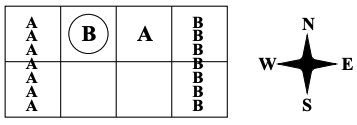
\includegraphics[scale=0.45]{figs/game-board}
    \caption{Soccer game, state s}
    \label{fig:game-board}
\end{figure}

The Soccer environment was implemented as a Python class with three main functions: \textit{get\_state}, \textit{simulate\_action} and \textit{render}. This structure was decided on after working with OpenAI's gym environment. The \textit{get\_state} function is trivial and simply returns a tuple of \textit{player A's position, player B's position, ball possession}. The \textit{render} function is also trivial and simply prints out (in the command line) a 4x2 grid show where the players are on the board and which player has the ball. The \textit{simulate\_action} actions as the transition function and can be seen in algorithm \ref{alg:soccer-env}

\begin{algorithm}
    \label{alg:soccer-env}
    \SetAlgoLined
    {\algorithmicindent} \textbf{Input} Player A's action, player B's action \\
    {\algorithmicindent} \textbf{Output} State, rewards vector, is\_terminal \\
    \If{Invalid action taken}{
        \textbf{return} current state, [0, 0], is\_terminal = False
    }
    Randomly select action order \\
    Apply first player's action and update their position \\
    \If{Player A's position matches Player B's position}{
        \If{Second player has possession}{
            Switch ball possession
        }
        \textbf{return} updated state, [0, 0], is\_terminal = False
    }
    Apply second player's action and update their position \\
    \If{Player A reached A goal with ball}{
        \textbf{return} updated state, [+100, -100], is\_terminal = True
    }
    \ElseIf{Player A reached B goal with ball}{
        \textbf{return} updated state, [-100, +100], is\_terminal = True
    }
    \ElseIf{Player B reached B goal with ball}{
        \textbf{return} updated state, [-100, +100], is\_terminal = True
    }
    \ElseIf{Player B reached A goal with ball}{
        \textbf{return} updated state, [+100, -100], is\_terminal = True
    }
    \textbf{return} updated state, [0, 0], is\_terminal = False
    \caption{Soccer environment's transition function - \textit{simulate\_action}}
\end{algorithm}

\subsection{Interfacing with the soccer environment}
The four experiments conducted on the soccer environment all revolved around the same basic setup, which can be seen in algorithm \ref{alg:training}. Where each algorithm varies is in the implementation of the function \textit{select\_epsilon\_greedy\_action}. The list of hyperparameter values can be see in table \ref{table:hyperparameters}. With these rates of decay, epsilon and alpha will reach their minimum at step 1,381,548. With a number of steps higher than this, neither the learning rate, nor the epsilon ever reach their minimum.

\begin{table}[]
    \label{table:hyperparameters}
    \caption{List of hyperparameters for training agent}
    \hline
    \begin{tabular}{ll}
    $\gamma$ & 0.9 \\
    $\epsilon$ & 1 \\
    $\epsilon$-decay & 0.000005 \\
    $\epsilon$-min & 0.001 \\
    $\alpha$ & 1 \\
    $\alpha$-decay & 0.001 \\
    $\alpha$-min & 0.000005 \\
    steps & 1000000 \\
    \end{tabular}
    \hline
\end{table}

\begin{algorithm}
    \label{alg:training}
    \SetAlgoLined
    Init Q-value table \\
    Init list of errors \doteq error\_list \\
    \For(){N number of steps}{
        Init soccer environment \doteq env \\
        \While(){True}{
            S \doteq env.get\_state() \\
            \overrightarrow{a} \doteq select\_epsilon\_greedy\_action \\
            S', R, done = env.simulate\_action(\overrightarrow{a}) \\
            record Q-value at state s \doteq before \\
            update Q-values using Bellman's equation \\
            record Q-value at state s \doteq after \\
            decay epsilon and learning rates \\
            error\_list.append(before - after) \\
        }
    }
    \textbf{return} error\_list \\
    \caption{Training an agent to learn the soccer environment}
\end{algorithm}

\section{Markov Games}
This soccer environment is an implementation of a Markov game - a stochastic game for which the probability transitions satisfy the Markov property\textsuperscript{1}. The optimal value function at state s (\textit{V*(s)}) is defined by maximizing the Q-value (\textit{Q*(s, a)}) over the action space. The actions that maximize the Q-values also define the deterministic optimal policy $\pi$*. This is illustrated in algorithm \ref{alg:optimal-policy}.

\begin{algorithm}
    \label{alg:optimal-policy}
    $\Pi$*(s) \in arg \max_{\overrightarrow{a} \in A\textsubscript{s}} Q\textsuperscript{*}(s, a)
\end{algorithm}

Markov games also define states slightly differently than the MDP we solved in project 2. Q-values are defined by stats and action vectors ($\overrightarrow{a}$), as opposed to state-action pairs. The Bellman equation changes only slightly as a result of this, adding n more dimensions, n being the number of players. Since there are only two players, this only increases the dimension of the Q-value table by 1.

\subsection{Nash equilibrium}
With this action vector, we can now approach optimizing this differently. We look for Nash equilibriums between the two players action spaces in order to optimize the overall reward. It helps to divide the Q-value dimension space into two parts for intuition.

Each Q-value is comprised of 5 dimensions: player A position, player B position, ball possession, player A action, player B action. We will dissect this state space in two parts. First, player position and ball possession are a reflection of the soccer environment, and so it requires no decision from the agent. Player position can have a value of {1..8}. Ball possession is a binary value: 0 indicates player B has the ball and 1 indicates player A has the ball.

For the action vector portion of the state space, each action can have a value of {1..5}. We can visualize this as a 5x5 grid, and discuss what an equilibrium looks like similarly to how the lecture videos discuss prisoners dilemma. In table \ref{table:prisoners-dilemma}, we see the Q-values across the action vector. This table have a Nash equilibrium for the action vector [down, down], since no player can increase their score given the other players action is fixed. This would not be the case for the action vector [right, left]. For this action vector, player B can increase their reward (from -100 to 0) be taking any other action. A similar argument can be made for the action vector [do nothing, up].

\begin{table}[]
    \label{table:prisoners-dilemma}
    \caption{Action vector state-space}
    \hline
    \begin{tabular}{lllll}
    0, 0 & 0, 0 & 0, 0 & 0, 0 & 0, 0 \\
    0, 0 & 0, 0 & 0, 0 & 100, -100 & 0, 0 \\
    0, 0 & 0, 0 & 60, 40 & 0, 0 & 0, 0 \\
    0, 0 & 0, 0 & 0, 0 & 0, 0 & 0, 0 \\
    -100, 100 & 0, 0 & 0, 0 & 0, 0 & 0, 0 \\
    \end{tabular}
    \hline
\end{table}

\subsection{Correlated-Q learning}
A correlated equilibrium is also a probability distribution, like Nash, with respect to one another's probabilities with added constraints. An important distinction between these two is that this correlated equilibrium can be computed easily via linear programming. In Greenwald and Hall, they illustrate these constraints with an example, using the game "chicken." Chicken is a two-player, two-action general-sum game. The reward structure can be seen below in figure \ref{fig:chicken-rewards}. The probability distribution of this action-vector always adds up to 1, and they are all non-negative. Further, rationality constraints are applied (see below in figure \ref{fig:chicken-rationality-constraints}). For intuition, we will talk through the first (upper-right) constraint from figure \ref{fig:chicken-rationality-constraints}: the probability of taking action L given action T ($\pi$\textsubscript{TL}) is less than or equal to half of taking action R given action T ($\pi$\textsubscript{RL}): 2$\pi$\textsubscript{TR} $\geq$ $\pi$\textsubscript{TL}.

\begin{figure}[]
    \centering
    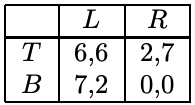
\includegraphics[scale=0.45]{figs/chicken-rewards.png}
    \caption{Chicken rewards}
    \label{fig:chicken-rewards}
\end{figure}

\begin{figure}[]
    \centering
    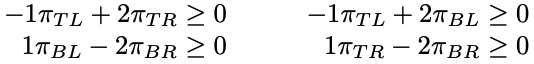
\includegraphics[scale=0.45]{figs/chicken-rationality-constraints.png}
    \caption{Chicken rationality constraints}
    \label{fig:chicken-rationality-constraints}
\end{figure}

\section{Q-Learning}
The off-policy Q-learning implementation here serves as our base-case to build from. The action selection here simply takes the max action from Q-value action space, relative to the Q-values of the player at hand. This essentially looks like the following: $\max_{a \in A\textsubscript{s}} Q(A position, B position, ball possession, a)$. This learner does not converge, as we can see in figure \ref{fig:q-learner}. The Q-value error acts sporadically for nearly all steps leading up to 1,000,000 steps. The line deceivingly looks like it converges toward the end. However, this is just simply the actions are being taken more deterministically.

As we can see here, this learner differs from the other 3 in that it does not evaluate the opponents action space in it's Q-values. For this reason, it makes no attempt to optimize it's Q-values based off of the other players available actions.

\begin{figure}[]
    \centering
    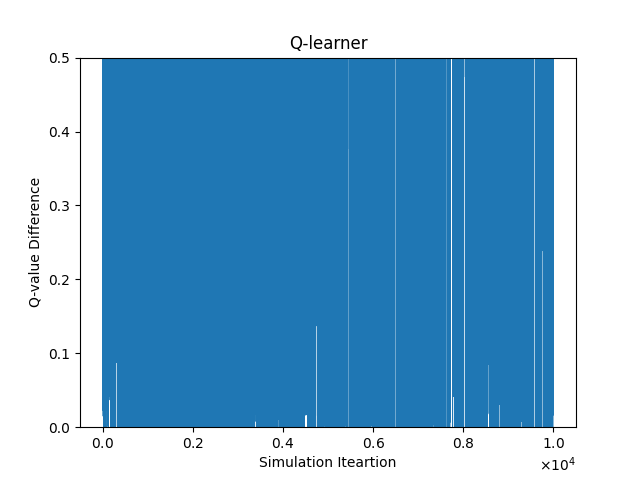
\includegraphics[scale=0.45]{figs/Q-learner}
    \caption{Q-learner performance measured by Q-value error}
    \label{fig:q-learner}
\end{figure}

\section{Friend-Q}
Greenwald and Hall implement Michael Littman's Friend-Q and Foe-Q learners here for comparison\textsuperscript{2}. The Friend-Q implementation is similar to our base Q-learner. The Q-value dimensions, as we see in algorithm \ref{alg:friend-q}, takes the max Q-value with consideration to both players actions. This will look like the following: $\max_{a\textsubscript{1} \in A\textsubscript{1}, a\textsubscript{2} \in A\textsubscript{2}} Q(A position, B position, ball possession, a\textsubscript{1}, a\textsubscript{2})$. Figure \ref{fig:friend-q} shows that the policy fails to converge as well. The Q-value errors falls to zero at around 80,000 steps.

\begin{algorithm}
    \label{alg:friend-q}
    V\textsubscript{i}(s) = \max_{a\textsubscript{1} \in A\textsubscript{1}, a\textsubscript{2} \in A\textsubscript{2}} Q\textsubscript{i}(s, a\textsubscript{1}, a\textsubscript{2})
    \caption{Friend-Q action selection\textsuperscript{2}}
\end{algorithm}

\begin{figure}[]
    \centering
    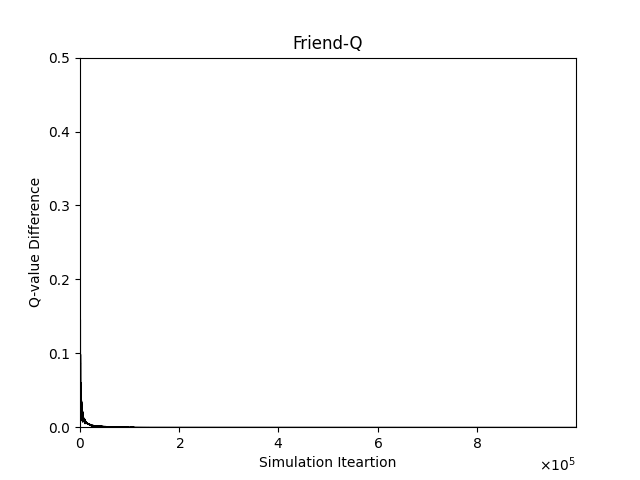
\includegraphics[scale=0.45]{figs/Friend-Q}
    \caption{Friend-Q performance measured by Q-value error}
    \label{fig:friend-q}
\end{figure}

\section{Foe-Q}
Foe-Q attempts to find an adversarial equilibrium. It is a slight modification of Friend-Q in that it attempts to maximize the Q-value over it's own action, while minimizing the Q-value over the opponents action. We see this change reflected in algorithm \ref{alg:foe-q}. This is when we first introduce cvxopt to solve this equilibrium with linear programming. This is an application of maximin (opposite of minimax from lecture).

The maximin linear programming portion of the \textit{select\_epsilon\_greedy\_action} function provides us with a probability distribution which we use to select an action. This will look like the following (using numpy): \textit{np.random.choice(np.arange(5), 1, p=probability\_distribution)}

After training the agent on Foe-Q for 1,000,000 steps, we can observe the Q-values for Q[2][1][1] (state s from figure \ref{fig:game-board}) in figure \ref{fig:foe-q-values}. This shows that it is most optimal for player A to take action 4. It also shows that Player A's expected reward goes down if player B takes action right and down. This follows intuition since we can expect a player B to have a direct line of sight to their goal in both of these scenarios. We also expect moving left to have a significant higher expected value since it is attempting to steal possession of the ball from player B.

\begin{algorithm}
    \label{alg:foe-q}
    V\textsubscript{1}(s) = \max_{\overrightarrow{a1} \in A\textsubscript{1}} \max_{\overrightarrow{a2} \in A\textsubscript{2}} Q\textsubscript{i}(s, \overrightarrow{a1}, \overrightarrow{a2}) = - V\textsubscript{2}(s)
    \caption{Foe-Q action selection}
\end{algorithm}

\begin{figure}[]
    \centering
    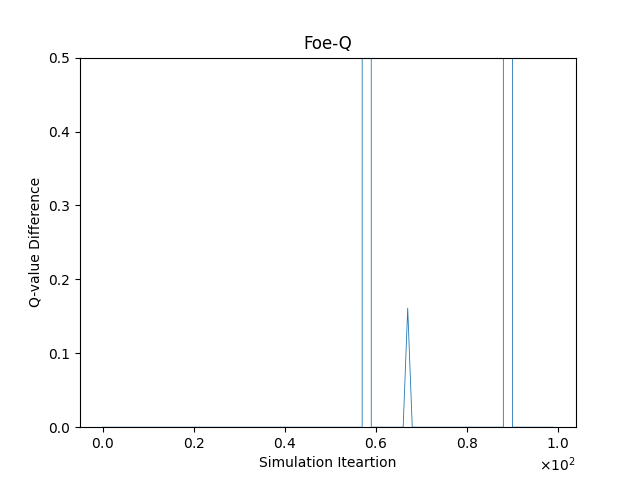
\includegraphics[scale=0.45]{figs/Foe-Q}
    \caption{Foe-Q performance measured by Q-value error}
    \label{fig:foe-q}
\end{figure}

\begin{figure}[]
    \centering
    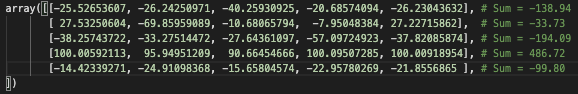
\includegraphics[scale=0.42]{figs/foe-q-values}
    \caption{Player 1 Q-value at state s from Foe-Q}
    \label{fig:foe-q-values}
\end{figure}

\section{Correlated-Q}
The correlated-Q (CE-Q) learner extends our linear programming portion of the learner from Foe-Q. However, outside of computing this probability distribution, the rest of the algorithm looks identical. Greenwald and Hall discuss four approaches to CE-Q.

\begin{figure}[]
    \centering
    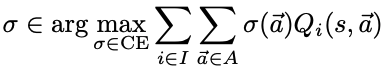
\includegraphics[scale=0.45]{figs/uCE-Q}
    \caption{Utilitarian CE-Q: maximize the sum of the players' rewards}
    \label{fig:uce-q}
\end{figure}

\begin{figure}[]
    \centering
    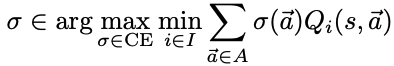
\includegraphics[scale=0.45]{figs/eCE-Q}
    \caption{Egalitarian CE-Q: maximize the minimum of the players' rewards}
    \label{fig:ece-q}
\end{figure}

\begin{figure}[]
    \centering
    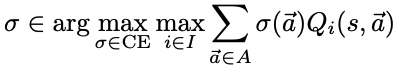
\includegraphics[scale=0.45]{figs/rCE-Q}
    \caption{Republican CE-Q: maximize the maximum of the players' rewards}
    \label{fig:rce-q}
\end{figure}

\begin{figure}[]
    \centering
    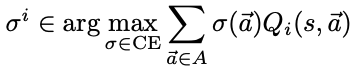
\includegraphics[scale=0.45]{figs/lCE-Q}
    \caption{Libertarian CE-Q: maximize the maximum of each individual payer i's rewards}
    \label{fig:lce-q}
\end{figure}

For our CE-Q learner, we implemented uCE-Q. We can see the algorithm, at a high level, in algorithm \ref{alg:ce-q}. The linear programming helper is attempting to maximize the sum of both of the player's rewards. At first thought, from a particle perspective, this didn't exactly make the most sense to me in a zero-sum game. In a real world application, it does not make sense to attempt to maximize your opponents reward, since this indirectly means minimizing your reward (zero sum). However, we can see after 1,000,000 steps, the Q-values offer much more insight to what the expected reward may be compared to Foe-Q.

See the Q-value distribution from CE-Q in figure \ref{fig:ce-q-values}. Let's dissect these Q-values and see if they provide more insight than those from Foe-Q. If player A knows what move player B will make, then the values that yield the highest value are the follow action vectors:

\begin{itemize}
    \item Player A: up, Player B: left $=>$ \textbf{100}
    \item Player A: right, Player B: left $=>$ \textbf{93}
    \item Player A: down, Player B: left $=>$ \textbf{93}
    \item Player A: left, Player B: left $=>$ \textbf{100}
    \item Player A: up, Player B: left $=>$ \textbf{100}
\end{itemize}

This is interesting, and offers some intricate insight that Foe-Q-values does not. It is stating that, under any situation, as long as player B goes left, it will result in a high reward for player A. Also, it states that if player A moves left, but player B moves right, it could lead to a very low reward. Foe-Q said otherwise (expected reward of 90). This makes a lot of sense, since this action vector would result in both players switching places, placing player B closer to their goal with the ball.

Figure \ref{fig:correlated-q} shows that CE-Q converges after about 800,000 steps, since each games error approaches zero, with an optimal policy. Greenwald and Hall point out that CE-Q eventually converges to a minimax equilibrium. We see this in our own results when reproducing these experiments.

\begin{figure}[]
    \centering
    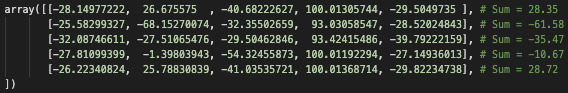
\includegraphics[scale=0.42]{figs/ce-q-values}
    \caption{Player 1 Q-value at state s from CE-Q}
    \label{fig:ce-q-values}
\end{figure}

\begin{algorithm}
    \label{alg:ce-q}
    V\textsubscript{i}(s) \in CE\textsubscript{i}(Q\textsubscript{1}(S), ..., Q\textsubscript{n}(s))
    \caption{Correlated-Q action selection}
\end{algorithm}

\begin{figure}[]
    \centering
    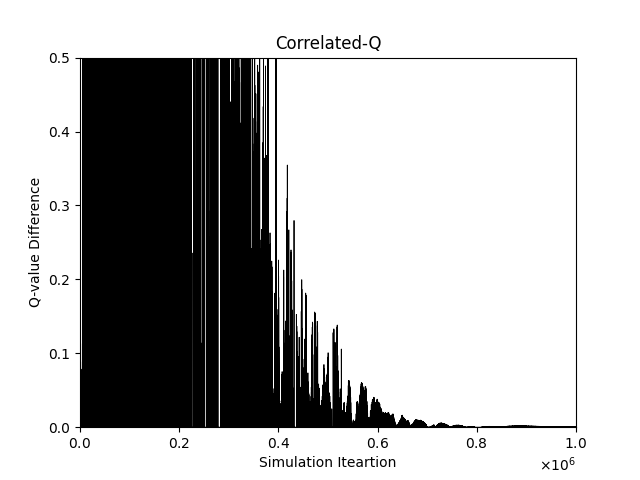
\includegraphics[scale=0.45]{figs/Correlated-Q}
    \caption{Correlated-Q performance measured by Q-value error}
    \label{fig:correlated-q}
\end{figure}

\section{Recapitulating Experiment Results}
We were able to get fairly close to the figures from Greenwald and Hall. Our results of Friend-Q are a little off in that the error approaches zero a lot quicker. The basic Q-learner is sporadic and matches the results fairly well. CE-Q and Foe-Q also converge similarly to Greenwald and Hall's results.

Reproducing these experiments were useful for gaining insight to how LP can help find these equilibriums. Tinkering with the Q-values, setting up the state-action space, and especially developing the Soccer environment all reflected useful real-world applications. Developing the soccer environment after having worked with the OpenAI environment was interesting to see how important it is to set up both sides of the learner.

\section{Pitfalls \& Problems}
One major issue when developing this was the runtime of the algorithm. The script takes several hours to complete, which made testing these algorithms very difficult. I typically tested this by only running it at about 100,000 - 300,000 steps in order to save time, then extrapolate to get an idea of how it will perform over all 1,000,000 steps. That way, when I eventually did run it at full length, I was able to do so with decent certainty that it would match the results of Greenwald and Hall.

One other issue was knowing how to properly unit test my LP helper function. To be able to isolate and unit test this, as well as the $\epsilon$-greedy action selection. I was able to unit test the soccer env pretty well. This was the first thing I did when starting out this project. This way, it was a tested and trusted portion of the code, and I didn't have to worry about this while working on the four Q-learner algorithms

\section{Further Research}
Given more time, I would have liked to experiment with a more rich reward structure. Developing a more elaborate environment gives you the ability to manipulate how the agent treats it's environment. Shaping these rewards in different ways will show insight on how you can get convergence faster. This was eluded to by Charles and Michael in the lecture series when they suggested that one easy way to find an equilibrium is to simply changes the rewards. This jokingly feels a little like cheating the system. However, when you build the system, you have the liberty to do this.

I would also like to explore and read more about the cvxopt library. The more experience and knowledge one gets around this API, the more one can leverage more intricate features. The linear algebra of the matrices and the solvers is also something that I would like to grasp a bit further.

\begin{thebibliography}{00}
\bibitem{b1} Amy Greenwald, Keith Hall, and Roberto Serrano. “Correlated Q-learning”. In: ICML. Vol. 20. 1. 2003, p. 242.
\bibitem{b2} M. Littman. Friend or foe Q-learning in general-sum Markov games. In Proceedings of Eighteenth International Conference on Machine Learning, pages 322–328, June 2001.
\end{thebibliography}

\end{document}
